%% bare_jrnl.tex
%% V1.4b
%% 2015/08/26
%% by Michael Shell
%% see http://www.michaelshell.org/
%% for current contact information.
%%
%% This is a skeleton file demonstrating the use of IEEEtran.cls
%% (requires IEEEtran.cls version 1.8b or later) with an IEEE
%% journal paper.
%%
%% Support sites:
%% http://www.michaelshell.org/tex/ieeetran/
%% http://www.ctan.org/pkg/ieeetran
%% and
%% http://www.ieee.org/


%%*************************************************************************
%% Legal Notice:
%% This code is offered as-is without any warranty either expressed or
%% implied; without even the implied warranty of MERCHANTABILITY or
%% FITNESS FOR A PARTICULAR PURPOSE! 
%% User assumes all risk.
%% In no event shall the IEEE or any contributor to this code be liable for
%% any damages or losses, including, but not limited to, incidental,
%% consequential, or any other damages, resulting from the use or misuse
%% of any information contained here.
%%
%% All comments are the opinions of their respective authors and are not
%% necessarily endorsed by the IEEE.
%%
%% This work is distributed under the LaTeX Project Public License (LPPL)
%% ( http://www.latex-project.org/ ) version 1.3, and may be freely used,
%% distributed and modified. A copy of the LPPL, version 1.3, is included
%% in the base LaTeX documentation of all distributions of LaTeX released
%% 2003/12/01 or later.
%% Retain all contribution notices and credits.
%% ** Modified files should be clearly indicated as such, including  **
%% ** renaming them and changing author support contact information. **
%%*************************************************************************


% *** Authors should verify (and, if needed, correct) their LaTeX system  ***
% *** with the testflow diagnostic prior to trusting their LaTeX platform ***
% *** with production work. The IEEE's font choices and paper sizes can   ***
% *** trigger bugs that do not appear when using other class files.       ***                          ***
% The testflow support page is at:
% http://www.michaelshell.org/tex/testflow/

%
\documentclass[conference]{pvsctran}
%
% If IEEEtran.cls has not been installed into the LaTeX system files,
% manually specify the path to it like:
% \documentclass[journal]{../sty/IEEEtran}

%\input epsf
\usepackage{graphicx}
\usepackage{hyperref}
\usepackage{graphicx}
\usepackage{amssymb}
\usepackage{amsmath}
\usepackage[super]{nth}
\usepackage{multicol}
% Add by Zhao
\usepackage{cite}
\usepackage{amsthm,amsfonts}
\usepackage{xcolor,color}
\usepackage{graphicx}
\usepackage{enumerate}
\usepackage{multirow}
\usepackage{subcaption}
\usepackage[utf8]{inputenc}
\usepackage[ruled]{algorithm2e}
\usepackage[colorinlistoftodos]{todonotes}


% correct bad hyphenation here
\hyphenation{op-tical net-works semi-conduc-tor}


\begin{document}

\title{ A Rapid Feasibility Checking for Reconfiguration of Mismatched PV Arrays}

\author{ \IEEEauthorblockN{\large Dafang Zhao, Fukohito Ooshita, and Michiko Inoue}
\IEEEauthorblockA{\large Nara Insititute of Science and Technology, Japan \\ Email:\{zhao.dafang.yu7, f-ooshita, kounoe\}@is.naist.jp}}

\setlength{\columnsep}{0.25in}


% make the title area
\maketitle


\begin{abstract}
%\boldmath
Power generation efficiency of photovoltaic (PV) arrays is significantly affected by partial shading and PV cell damage. Partial shading or PV cell damage induces mismatched power generation among PV panels and causes an efficiency loss of power generation. Power generation of mismatched PV arrays can be recovered by reconfiguring connection of PV panels. 
In this paper, we introduce a \textit{feasibility check problem} of PV panel configuration.
The problem identifies whether a connection among PV panels can be configured from a given PV module level solution. 
We also propose an algorithm for the feasibility check problem. The experimental results demonstrate that the proposed method can identify feasible configurations more than 32,000X faster than the exhaustive search with around 0.6\% errors. 
\end{abstract}

\begin{IEEEkeywords}
photovoltaic, feasibility, reconfiguration, mismatch
\end{IEEEkeywords}

\IEEEpeerreviewmaketitle



\section{Introduction}
As fossil fuel depletion and environmental pollution become more serious, green and renewable energy has become necessary for a sustainable society and environment. 
Photovoltaic (PV) systems receive significant attention since the sun has unlimited energy and PV arrays can be easily scaled up. 
However, due to the nature of a PV cell, which is a basic component of a PV array, PV arrays are sensitive to partial shading and PV cell damage. 
PV cells could not uniformly generate power when PV cells experience different irradiances or some of cells have physical defects, and such a mismatched condition might accelerate heating and aging of PV cells and cause further damaging. 
To prevent PV cells from damaging, bypass diodes are usually placed in PV arrays and they are turned on in mismatched conditions. 
However, it causes a significant loss of power generation. 

PV arrays are hierarchically constructed such that a group of PV cells form a PV module, a group of PV modules form a PV panel, and a group of PV panels form a PV array. 
Power generation of mismatched PV arrays can be recovered by reconfiguring connection of these components. 
Fig.\ref{compare} shows an example of power generations of a PV array with a partial shading. 
We distributed shading cells non-uniformly to a PV array with 3 $\times$  4 PV panels and applied power simulation. 
Before reconfiguration, it has four peaks in power VS voltage curve, while,  if we reconfigure connection among PV panels, it can increase around 35\% power generation.

Though several reconfiguration methods have been proposed, most works consider reconfiguration in PV cell or PV module level \cite{nguyen2008adaptive,wang2014architecture,storey2013improved,storey2014optimized,udenze2018reconfiguration}. 
However, cell level reconfiguration requires a significantly high computation time and a large number of switches for reconfiguration. 
In addition, they require a special PV panels with capability of switching, and cannot be applied to the system constructed with standard PV panels. 
From a practical view, reconfiguration of connection among PV panels is a realistic solution since a PV panel is manufactured as a physical one panel with two terminals and PV panels can be flexibly interconnected. 
\begin{figure}[t]
    \centering
    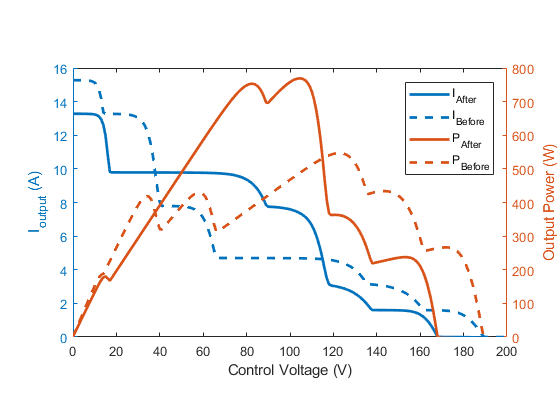
\includegraphics[width=0.8\linewidth]{PVSC-46/fig/compare.png}
    \caption{Power generation before and after reconfiguration}
    \label{compare}
\end{figure}

Reconfiguration in PV panel level has been investigated\cite{carotenuto2015evolutionary,hu2017non,orozco2016optimized}. 
A PV array reconfiguration using genetic algorithm (GA) was proposed in \cite{carotenuto2015evolutionary}. Though it can give a new configuration, computing cost is significantly high and the algorithm cannot generate the best configuration precisely.  
Hu et al. also addressed PV panel reconfiguration where they formulate a nonlinear integer programming problem to optimize power generation by reconfiguration \cite{hu2017non}.
Orozco-Gutierrez et al. proposed an efficient and effective reconfiguration method\cite{orozco2016optimized} where it first selects candidates of configurations with approximation and then finds the best one with precise power simulation. 
However, the candidates are specified in a PV module level though PV modules could not be fully reconfigured. Actually, we found that some of configuration candidates are not able to be realized. However, the paper\cite{orozco2016optimized}  does not show any systematic way to identify such a feasibility. 

In this paper, we propose an algorithm to rapidly check feasibility that a given configuration candidate is actually formed by given PV panels. 
The proposed method can efficiently check the feasibility while identifying most feasible cases accurately. 
The experimental results demonstrate the effectiveness of the proposed method can identify the feasibility of configurations and false negative are less than 1\%.





\section{Photovoltaic Array}

A PV system or PV array is composed of PV panels that have two terminals of plus and minus and can be interconnected.
There are two common connection styles for PV arrays, \textit{series-parallel} array and \textit{total-cross-tied} array. 
In a series-parallel array, PV panels are connected in series, and multiple series connections are connected in parallel. 
In a total-cross-tied array, parallel connections of PV panels are connected in series. 
In this paper, we focus on series-parallel arrays, however the basic idea of the proposed method can be applied also to total-cross-tied arrays. 
Hereafter, we simply call a series-parallel array a \textit{PV array}. 

Figure \ref{model} shows an example of a PV array. 
A PV array is a parallel connection of (PV) strings where a string is a series connection of PV panels. 
A PV panel is a series connection of PV modules, and a PV module is a parallel connection of a series of PV cells and a bypass diode. 
A typical PV panel is composed of three PV modules each of which has 12-24 PV cells. 
A PV module can generate power for a given voltage according to its I-V characteristics as shown in Fig.\ref{fig:IV}(a - c). 
The I-V characteristics is affected by irradiance level and physical damage of PV cells. 
Figure \ref{fig:IV}(a) also shows a typical degradation of a I-V characteristics where generated current is reduced with some ratio while keeping the voltage range. 
When a PV panel has a partial shade, that is its PV modules have different irradiance levels and hence different I-V characteristics, the PV panels might have multiple peaks (maximum power points, MPPs) in power generation as shown in Fig.\ref{fig:IV}(d). 

To find out accurate I-V characteristics of a PV panel, we need a time consuming power simulation. 
However, we can roughly understand I-V characteristics of a PV panel (and also a string) as follows. 
When a control voltage is low, PV modules with high irradiance level are active while PV modules with low irradiance level are inactive with turning on their bypass diodes.
In this case, a high current can flow in the PV panel. When control voltage is high, some of bypass diodes become turning off and the corresponding PV modules become active. 
In this case, the current level is reduced and generated power sometimes increases and sometimes decreases. 
The generated power at MPPs can be roughly estimated. 
In Fig.\ref{fig:IV}(d), one PV panel has three PV modules with different irradiance levels. 
The peak currents for these modules are 433mA, 307mA, and 155mA, respectively. 
Voltages at MPPs are roughly 200V, 400V, 600V in Fig.\ref{fig:IV}(d), those are roughly multiples of a voltage of MPP for one PV module (around 200V in this case). 
At the first MPP (MPP1), only one PV module with a peak current of 433mA is active at a control voltage of 206V, so the generated power is 89W. 
At the second MPP (MPP2), two PV modules with peak currents of 433mA and 307mA are active at a control voltage of 420V. 
In this case, the current level of the PV panel is 307mA since two PV panels are connected in series and they have to have the same current level, and the generated power is 129W. At the third MPP (MPP3), the current level of the PV panel is 155mA at a control voltage of 644V, and the generated power is 100W. 

In a PV array, we have two constraints. 
PV panels in the same string have the same current level, while all the strings have the same control voltage. 
When considering reconfiguration of PV panel connection, we should find out the best configuration while considering these constraints. 

\begin{figure}[t]
    \centering
    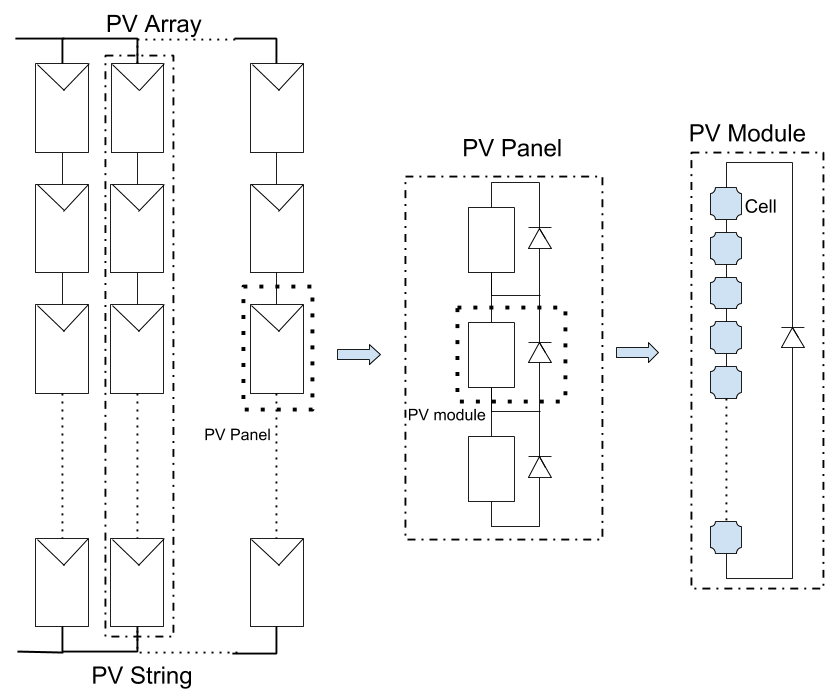
\includegraphics[width=0.8\linewidth]{module.png}
    \caption{PV array, string, module and panel}
    \label{model}
\end{figure}

\begin{figure}
     \centering
    \begin{subfigure}[b]{0.3\linewidth}
        \centering
        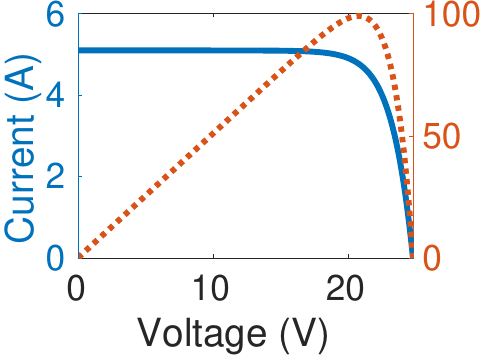
\includegraphics[width=\linewidth]{PVSC-46/fig/m_1.png}
        \caption{PV module 1}
     \end{subfigure}
     \begin{subfigure}[b]{0.3\linewidth}
        \centering
        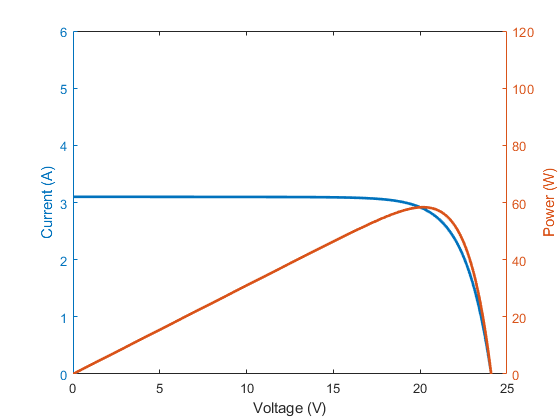
\includegraphics[width=\linewidth]{PVSC-46/fig/m_2.png}
        \caption{PV module 2}
     \end{subfigure}
     \begin{subfigure}[b]{0.3\linewidth}
        \centering
        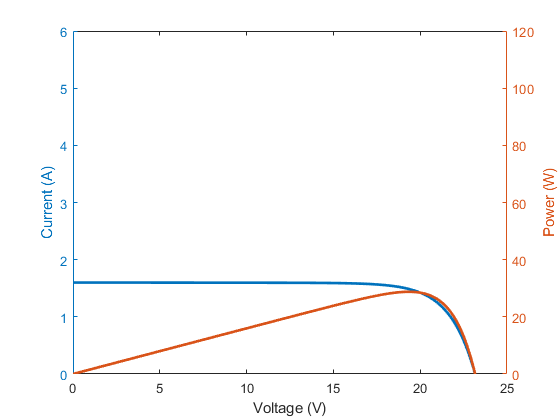
\includegraphics[width=\linewidth]{PVSC-46/fig/m_3.png}
        \caption{PV module 3}
    \end{subfigure}
    \hfill
    \begin{subfigure}[b]{\linewidth}
        \centering
        \vspace{3mm}
        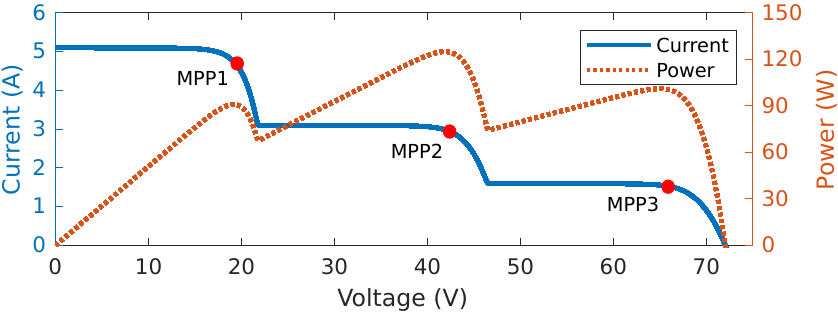
\includegraphics[width=\linewidth]{PVSC-46/fig/panel.png}
        \caption{PV panel}
    \end{subfigure}
    \caption{I-V characteristics}
    \label{fig:IV}
\end{figure}
% \subsection{ Major Subsections}
% As shown, denote subsections with left justified 10-point Times Italic. Order them with capitalized alphabetic characters $(A, B,...)$. Follow the letter designation with a period, a single space, and then the subsection title capitalizing the first letter of each word. The paragraph description of the subsection heading is set to "exactly 12-point" line spacing with 6 points before and after.
% \subsection{ Equations }
% Equations should be centered in the column and numbered sequentially. Place the equation number to the right of the equation within a parenthesis, with right justification within its column. An example would be
% \begin{equation}
% V_{OC}=\frac{1}{\beta}ln\left(\frac{I_L}{I_S}+1\right)
% \end{equation}
% \emph{Make sure that any subscripts in your equations are legible and are not too
% small to read!} When referring to an equation, use the number within
% parenthesis. For example, you would usually refer to the first
% equation as (1) rather than equation (1). If possible, use the Symbol
% font for all special characters.%, or better yet, use Equation Editor or
% %MathType. 
% The paragraph description of the line containing the
% equation should be set for 6 points before and 6 points after. The
% paragraph spacing will need to be set to ``single'' rather than ``exactly
% 12 point'' so that the height will autoscale to fit the equation.

% \section{Figures and Tables}
% The use of color in figures and photos is recommended.  Keep in mind that the proceedings will only be produced in electronic format (DVD).  There will not be a hardbound version of the proceedings.  Please consider the use of different line styles (dashes, dots, etc.) in plots to ensure clarity.  See example.  Please use jpg or png format for all images and compress the size.

% Most of the following applies to Microsoft Word.  Figures should utilize as much of the column width as possible in order to maximize legibility. Use a sans serif font, such as Helvetica. Helvetica is larger and much easier to read than Times. Using 8- to 10-point Helvetica usually results in a legible figure. \emph{Do not use any font smaller than 8-point!} It must be legible. When referring to a figure, use the abbreviation Fig. followed by its number. Place figure captions directly below each figure. Use
% 9-point Times with the paragraph spacing set at ``exactly 10 points.'' Set a tab at 0.5 inch. Type ``Fig. \#.'' (\# is the numeral) then tab over to the 0.5 inch mark before beginning the text of the figure caption. Note that figure captions are always (left and right) justified, rather than centered, even if they are less than a single full line in length. See the caption for Fig. 1.

% Within \LaTeX, there is basically only one option for placing figures
% within your paper.  Often the easiest way is to insert them into the
% top of the next column.
%Within Microsoft Word there are several options for placing figures
%within your paper. Often the easiest is to insert them between
%existing paragraphs allowing the figures to remain in that relative
%position. The paragraph description where the figure is inserted must
%be set to ``single'' spacing rather than ``exactly 12 points'' in
%order to allow the line to autoscale in height to display the entire
%figure. Some disadvantages of this approach are that you don't have
%total flexibility in placing figures, and that the figures will move
%as text is inserted or deleted in any part of the document before the
%figure. If you elect to use this approach, it is recommended that you
%nearly complete the editing of your text before inserting any
%figures. Remember to allow room for them, however. Then begin
%inserting figures starting from the beginning of your document. 
% Do not lump all figures at the end of the paper!
% If you have difficulties with the titles on your figures, you can always elect to add in the titles as separate text boxes, rather than importing the titles with the graph. This is sometimes helpful in getting a lengthy vertically-oriented title to display correctly.

% %\begin{figure}
% %%\includegraphics {figure_temp.epsi}
% %\epsfxsize=3.25in\epsfbox{figure1.eps}
% %\caption{ Estimated relationship between the time an author spends reading these instructions and the quality of the author's digest article.}
% %\end{figure}

% \begin{figure}
% \centering
% 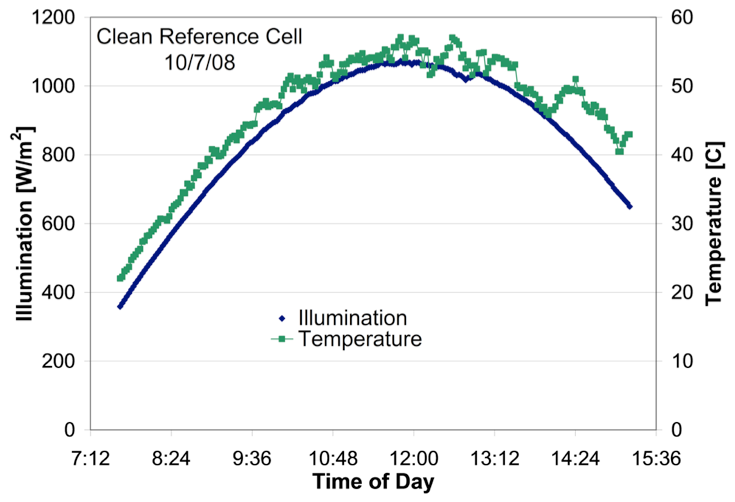
\includegraphics[width=9cm]{image1.png}
% \caption{Example of readable plot using different colors and line styles for clarity.}
% \end{figure}

% Notice that prior to the graph, a single 12-point line is used to
% separate the preceding text from the graph. The equivalent of a blank
% line should exist between the bottom of the graph (the x-axis caption)
% and the figure caption. (In this particular case, there was no need to
% add a blank line between the x-axis label and the figure caption,
% because there was already adequate spacing provided by the image
% border.) After the figure caption, there should be a single 12-point
% blank line before the text resumes. 
%\LaTeX accepts encapsulated post script files as figures.  Standard post script figures will not expand and contract to fill the designate area on the page. Encapsulated post script files will.  Thus, encapsulated post script files must obviously be only one page long.  It is often easy to convert a post script file to encapsulated post script.  In Linux this can be done with the command, ``ps2epsi.''
%More flexibility is obtained in inserting figures if you can place
%them exactly where you would like them to be on a page. This can be
%accomplished by inserting the figure, selecting the figure, and then
%choosing ``Format Picture\dots ''. Various settings allow you to place the figure at an absolute position on a page; specify if the text is supposed to flow around the figure or if the figure should move with the text, etc. If you elect to let the text flow around the figure, then remember that you will have to insert a separate text box for the caption, otherwise the figure caption is likely to become separated from the figure.
%When importing a graph from Excel into Word, it is often helpful to
%special-paste it in as a ``Picture (Enhanced Meta-file).'' This saves
%file memory for Word documents. Be aware that the usual Copy
%$\rightarrow $  Paste procedure will copy the entire Excel spreadsheet into your Word file. The Copy $\rightarrow$ Paste Special $\rightarrow$ Picture (Enhanced Metafile) command copies only the graph as a static picture. This is not a concern with PDF file submissions.
% If you decide to use color traces in your graphical data, be absolutely certain that there is no ambiguity about your graphical information when printed on a B\&W printer.

% Table I on the second page was inserted using ``Insert'', ``Text
% Box'', creating the text contained in Table I, and then formatting the
% text box using all the settings available under ``Format'', ``Text
% Box\dots ''. Table I also serves as an illustration of one of the rare
% instances when the double column format requirement can be
% violated. Certain figures and tables will require the full-page width
% to display. It is usually best to place these figures and tables at
% the top, rather than in the middle or bottom of a page. Tables should be entered within a single column if this can be done cleanly, without the entry becoming too crowded.

% \section{Citing Previous Work}
% When referencing a journal article \cite{Yamaguchi}, a conference
% digest article \cite{Hovel} or a book \cite{Fahrenbruch}, place the reference numbers within square
% brackets. To simultaneously cite these references \cite{Yamaguchi} - \cite{Fahrenbruch} use the format just demonstrated. The reference list is the last section and references are listed in the order cited. Use 9 point Times. The paragraph description is set for a line spacing of exactly 10 points with 0 point spacing before and after. A 0.25 inch hanging indention should be specified. 

% Generally speaking, references should be very detailed. For journal articles, list all authors by initials and last name, the title of the paper in quotations (capitalizing only the first letter of the first word, unless it would be capitalized in a sentence, e.g., a proper noun), the journal name in italics, the volume number, the issue number, the page numbers, and the date. Use the examples provided \cite{Yamaguchi} - \cite{Fahrenbruch} as a guide. 
% %Further information on LaTeX and TeX can be found in \cite{IEEEhowto:kopka} - \cite{knuth}. 

% % The following statement makes the two columns on the last page more
% % or less of equal length.  Placement of this command is by trial and error.
% \vfil\eject

% \section{Copyright and Reprint Information}
% The IEEE copyright form will be electronically submitted for this conference.  On the conference web site, follow the link in the manuscript submission area. 

% Reprints may be ordered by checking the appropriate box on the conference registration form.  The reprints will be mailed to you at the address listed on the registration form approximately 3 months after the conference.


\section{Conclusion}
Following these instructions will improve the quality of your paper and the PVSC Proceedings. If you have comments, please contact \url{Publications@ieee-pvsc.org}. Please direct questions regarding the electronic submission process to \url{help@SPLTrak.com}. 

% conference papers do not normally have an appendix

% use section* for acknowledgment



% conference papers do not normally have an appendix


% use section* for acknowledgement



% trigger a \newpage just before the given reference
% number - used to balance the columns on the last page
% adjust value as needed - may need to be readjusted if
% the document is modified later
%\IEEEtriggeratref{8}
% The "triggered" command can be changed if desired:
%\IEEEtriggercmd{\enlargethispage{-5in}}

% references section
\renewcommand\refname{Reference}
\bibliographystyle{ieeetr}
\bibliography{reference}
% can use a bibliography generated by BibTeX as a .bbl file
% BibTeX documentation can be easily obtained at:
% http://www.ctan.org/tex-archive/biblio/bibtex/contrib/doc/
% The IEEEtran BibTeX style support page is at:
% http://www.michaelshell.org/tex/ieeetran/bibtex/
%\bibliographystyle{IEEEtran}
% argument is your BibTeX string definitions and bibliography database(s)
%\bibliography{IEEEabrv,../bib/paper}
%
% <OR> manually copy in the resultant .bbl file
% set second argument of \begin to the number of references
% (used to reserve space for the reference number labels box)
% \begin{thebibliography}{1}
% \small

% \bibitem {Yamaguchi}
% M. Yamaguchi, A. Khan, S.J. Taylor, M. Imaizumi, T. Hisamatsu, and S. Matsuda, ``A detailed model to improve the radiation-resistance of Si space solar cells,\emph{Fundamentals of Solar Cells} vol. 46, pp. 2133-2138, 1999.

% \bibitem {Hovel}
% H. J. Hovel and J. M. Woodall, ``The effect of depletion region recombination currents on the efficiencies of Si and GaAs solar cells'', \emph {in 10th IEEE Photovoltaic Specialist Conference}, p. 25, 1973.

% \bibitem {Fahrenbruch}
% A. L. Fahrenbruch and R. H. Bube, \emph{Fundamentals of Solar Cells}, New York: Academic Press, 1983.

% %\bibitem{IEEEhowto:kopka}
% %H.~Kopka and P.~W. Daly, \emph{A Guide to \LaTeX}, 3rd~ed.\hskip 1em plus
% %  0.5em minus 0.4em\relax Harlow, England: Addison-Wesley, 1999.

% \end{thebibliography}
%\smallskip
%Note: For the Summary paper submission only, references to the authors own work must be redacted to preserve the new double-blind reviewing requirements.





% that's all folks
\end{document}


